\documentclass[12pt,a4paper,twoside,openright]{report}
\usepackage[utf8]{inputenc}
\usepackage[T1]{fontenc}
\usepackage{geometry}
\geometry{top=1.2in,bottom=1.5in,inner=1.5in,outer=1in,footskip=0.5in}
\usepackage{lmodern}
\usepackage{graphicx}
\usepackage{setspace}
\usepackage{amsmath,amssymb,amsfonts}
\usepackage{booktabs,tabularx,array,multirow}
\usepackage{enumitem,multicol}
\usepackage{microtype}
\usepackage{tikz}
\usetikzlibrary{arrows.meta,positioning,fit,calc}
\usepackage{titlesec}
\usepackage{caption}
\usepackage{float}
\usepackage{epstopdf}
\usepackage{ragged2e}
\usepackage{hyperref}

\widowpenalty=10000
\clubpenalty=10000
\raggedbottom
\setlength{\emergencystretch}{2em}

\hypersetup{
  colorlinks=true,
  linkcolor=black,
  filecolor=black,
  urlcolor=blue,
  citecolor=black
}

\titleformat{\chapter}[display]
  {\normalfont\bfseries\raggedleft}
  {\fontsize{100}{110}\selectfont\thechapter}
  {-15pt}
  {\Huge}

\titleformat{name=\chapter,numberless}[block]
  {\normalfont\bfseries\Huge\centering}
  {}
  {0pt}
  {}

\newcolumntype{Y}{>{\raggedright\arraybackslash}X}
\newcolumntype{P}[1]{>{\raggedright\arraybackslash}p{#1}}
\newcommand{\projecttitle}{Placement-Aware Dynamic Graph Learning for Robust Wearable Human Activity Recognition}
\newcommand{\studentname}{Prabhat Kumar}
\newcommand{\rollnumber}{2022-IMT-086}
\newcommand{\supervisorname}{Dr. Anjali}

\begin{document}
\setstretch{1.5}

\hypersetup{pageanchor=false}
\begin{titlepage}
\begin{center}
\fontsize{15.8pt}{19pt}\selectfont
\textbf{\projecttitle}

\vspace*{0.13in}
\emph{\large Residual Adaptive Sensor Routing under Placement Shift}

\vspace*{0.35in}
{\large An M.Tech Major Project Report submitted\par}
{\large in partial fulfilment of the requirements for the degree of\par}
{\large Integrated Post Graduate (M.Tech.) in Information Technology\par}

\vspace*{0.4in}
{\large submitted by\par}
{\large\textbf{\studentname\ : \rollnumber}\par}

\vspace*{0.3in}
{\large Under the Supervision of\par}
{\large\textbf{\supervisorname}\par}

\vspace*{0.3in}
{\large Department of Information Technology\par}

\vfill
{\large ABV-INDIAN INSTITUTE OF INFORMATION TECHNOLOGY\par}
{\large AND MANAGEMENT GWALIOR\par}
\vspace*{0.05in}
{\large GWALIOR, MADHYA PRADESH, INDIA\par}
\vspace*{0.05in}
{\large OCTOBER 2026\par}
\end{center}
\end{titlepage}

\cleardoublepage
\hypersetup{pageanchor=true}
\pagenumbering{roman}
\setcounter{page}{1}

\chapter*{Candidate's Declaration}
\addcontentsline{toc}{chapter}{Candidate's Declaration}
\vspace{0.5cm}
\noindent
I, \studentname\ (\rollnumber), a student of the Integrated B.Tech. + M.Tech. programme of ABV-IIITM Gwalior, declare that the work presented in this Major Project report has been prepared by me under the supervision of \supervisorname. It presents the completed Summer Colloquium as prior work and the dynamic-graph study as proposed work. Due credit has been given to the original authors and sources for all words, ideas, methods, datasets, diagrams, software and results that are not my original contribution. Proposed experiments are not represented as completed results.

\vspace{1.5cm}
\begin{center}
\begin{tabular}{p{0.54\textwidth}p{0.36\textwidth}}
Date: & \textbf{Signature of Candidate:} \\[0.4cm]
\studentname\ (\rollnumber) & \\
\end{tabular}
\end{center}

\vspace{1.5cm}
\noindent This is to certify that the above statement made by the candidate is correct to the best of my knowledge.

\vspace{1.2cm}
\begin{center}
\begin{tabular}{p{0.54\textwidth}p{0.36\textwidth}}
Date: & \textbf{Signature of Supervisor:} \\[0.4cm]
& \supervisorname \\
\end{tabular}
\end{center}

\cleardoublepage
\chapter*{Acknowledgement}
\addcontentsline{toc}{chapter}{Acknowledgement}
\vspace{0.5cm}
\noindent
I express my sincere gratitude to \supervisorname\ for the guidance and discussions that shaped the transition from the Summer Colloquium to the present research direction. I also thank the Department of Information Technology, ABV-IIITM Gwalior, for providing the academic environment and computational facilities needed for this work. Finally, I thank my family and friends for their constant encouragement and support.

\vspace{1cm}
\begin{flushright}
\textit{\textbf{\studentname}}\\
\textit{\textbf{\rollnumber}}
\end{flushright}

\cleardoublepage
\chapter*{Abstract}
\addcontentsline{toc}{chapter}{Abstract}
\vspace{0.5cm}
\noindent
Multi-sensor wearable human activity recognition (WHAR) can be modelled as a graph in which body-worn inertial measurement units form nodes and inter-sensor relationships form edges. The completed Summer Colloquium progressed from a GT-WHAR-inspired graph--BiGRU baseline to GAE--Mamba--WHAR, combining a graph-autoencoder objective, sensor-drop training and a lower-latency temporal replacement. That study reported improved robustness to simulated dead sensors and reduced batch-level GPU inference time, but the anatomical graph remained fixed and REALDISP evaluation focused on ideal placement. A missing sensor and a displaced sensor are different: a displaced sensor remains active but may provide measurements in a changed reference frame or from a shifted position.

This project therefore proposes placement-aware dynamic routing. The central question is whether input-dependent, availability-aware edges can reduce cross-placement macro-F1 degradation beyond a corrected fixed graph, rotation/dropout augmentation and an existing dynamic wearable baseline. The proposed model forms per-IMU embeddings and combines three graph components: a physical anatomical prior, a globally learned graph and a sample-dependent affinity graph. Weighted message passing is followed by a verified temporal backbone and activity classifier. The inherited reconstruction decoder is retained only if controlled ablation shows that it improves recognition.

The methodology is grounded primarily in GT-WHAR, DynamicWHAR, 2s-AGCN, Mamba, DecomposeWHAR and the REALDISP displacement study. REALDISP is the primary dataset; DSADS is secondary and OPPORTUNITY is retained only for limited supplementary evaluation. The planned protocol uses subject-separated splits, training-only normalization, matched baselines, branch ablations, macro-F1, clean-to-shift degradation and batch-one efficiency measurements. No new dynamic-graph result is claimed at this proposal stage. The intended contribution is a reproducible test of residual placement-aware routing for the completed Summer Colloquium system.

\textbf{Keywords:} wearable human activity recognition, inertial measurement unit, dynamic graph, sensor displacement, adaptive routing, REALDISP, state-space model.

\cleardoublepage
\tableofcontents
\cleardoublepage
\listoffigures
\addcontentsline{toc}{chapter}{List of Figures}
\cleardoublepage
\listoftables
\addcontentsline{toc}{chapter}{List of Tables}

\cleardoublepage
\chapter*{List of Abbreviations}
\addcontentsline{toc}{chapter}{List of Abbreviations}
\begin{center}
\begin{minipage}{0.82\textwidth}
\begin{tabularx}{\textwidth}{@{}P{0.22\textwidth}Y@{}}
AGCN & Adaptive Graph Convolutional Network \\
BiGRU & Bidirectional Gated Recurrent Unit \\
GAE & Graph Autoencoder \\
GIN & Graph Isomorphism Network \\
HAR & Human Activity Recognition \\
IMU & Inertial Measurement Unit \\
LOSO & Leave-One-Subject-Out \\
SSM & State-Space Model \\
WHAR & Wearable Human Activity Recognition \\
\end{tabularx}
\end{minipage}
\end{center}

\cleardoublepage
\pagenumbering{arabic}

\cleardoublepage
\chapter{Introduction}

This chapter introduces the research context, explains the motivation for moving from sensor-failure robustness to placement robustness, and provides the background required for the proposed study. It closes with the scope, objectives, expected contributions and organisation of the report.

\section{Context}
Wearable human activity recognition uses body-worn sensors to infer activities such as walking, sitting, exercising and performing daily tasks. An inertial measurement unit commonly provides tri-axial acceleration, angular velocity and magnetic-field measurements. Wearable sensing is attractive for rehabilitation, assisted living, sports monitoring and occupational safety because it can operate continuously without a fixed camera or controlled field of view.

Deep learning allows representations to be learned directly from multivariate sensor windows. DeepConvLSTM combines convolutional feature extraction with recurrent temporal modelling and remains a standard non-graph reference~\cite{deepconvlstm}. In a multi-IMU system, however, sensors are not merely channels: their body locations have meaningful relationships. A wrist and an ankle observe different local motion, yet their measurements are connected through the activity and the body's kinematic structure.

Graph neural networks provide a natural representation of this setting. Sensors are modelled as nodes, inter-sensor relationships as edges, and message passing combines complementary information. GT-WHAR presents a graph-based temporal framework for multiple wearable sensors~\cite{gtwhar}. The student's completed Summer Colloquium began from this direction and developed GAE--Mamba--WHAR~\cite{summerreport}.

\section{Motivation}
The Summer Colloquium addressed two practical concerns: temporal inference cost and recognition when sensors become unavailable. Sensor-drop training and an auxiliary graph reconstruction objective were used to increase robustness when one or more sensor streams were removed. The next limitation is different. In daily use, a sensor may be attached with an orientation offset or shifted locally from its intended position. It remains active and produces a signal, but the distribution and inter-sensor relationship may change.

A fixed anatomical graph assumes that the same connections are valid for every subject, activity and attachment condition. This prior can be useful under correct placement, but it cannot change its edge strengths according to the observed movement. A completely unconstrained learned graph is flexible, yet may ignore valuable anatomical structure or overfit the limited displaced recordings. This motivates a residual graph that keeps the physical prior and learns only the corrections required by the data.

The problem also requires precise terminology. Orientation change, local placement shift, missing sensors and software-level channel permutations are not equivalent. Orientation changes transform vector axes; local shift changes the motion measured at the device; failure removes a measurement; and permutation changes input identity without modelling physical relocation. The study therefore evaluates these conditions separately and uses recorded REALDISP placement scenarios as primary evidence~\cite{banos,realdisp}.

\section{Background}

\subsection{Wearable Activity Recognition}
A multi-sensor window is represented as $X\in\mathbb{R}^{T\times N\times F}$, where $T$ is the number of samples, $N$ the number of IMUs and $F$ the features per sensor. A classifier maps $X$ to one of $C$ activity labels. Performance depends not only on the model but also on windowing, label policy, subject splits, normalization and metric choice.

Subject-independent evaluation is essential. Test subjects must not contribute windows or preprocessing statistics to training. Accuracy alone may hide minority-class failures; macro-F1, per-class results and clean-to-shift degradation provide a more informative robustness picture.

\subsection{Graph-Based Multi-Sensor Recognition}
For a graph $G=(V,E)$, $V$ is the set of sensor nodes, $E$ is the set of inter-sensor edges, and $v_i\in V$ denotes sensor $i$. A simple weighted graph layer is
\[
H^{(\ell+1)}=\sigma\!\left(AH^{(\ell)}W^{(\ell)}\right),
\]
Here, $H^{(\ell)}$ and $H^{(\ell+1)}$ are the node-feature matrices before and after graph layer $\ell$, $A$ is the weighted adjacency matrix, $W^{(\ell)}$ is the trainable feature transformation and $\sigma(\cdot)$ is a nonlinear activation. A fixed $A$ expresses a predetermined topology; a dynamic $A(X)$ changes with input window $X$ or its latent features.

Graph Isomorphism Networks use expressive neighbourhood aggregation~\cite{gin}. GT-WHAR combines graph processing with temporal modelling for wearable signals~\cite{gtwhar}. The present proposal retains this spatial--temporal decomposition but changes how spatial connections are constructed.

\subsection{State-Space Temporal Modelling}
Recurrent networks process sequences step by step, which can limit parallelism. Mamba introduces input-dependent selective state-space parameters and a hardware-aware scan~\cite{mamba}. It motivates efficient temporal modelling but does not itself provide sensor placement invariance. The graph and temporal components must therefore be evaluated separately.

\section{Scope}
The primary scope is recorded orientation and local placement variation represented by REALDISP. Sensor dropout and synthetic rotations are controlled stress tests. Arbitrary relocation from one body part to another is outside the main claim because dynamic attention alone cannot identify the true anatomical location of an unknown device.

The proposed graph is an inference-time routing mechanism: it recomputes edge weights from the current input. It does not update model parameters online. The report also does not claim smartwatch deployment; efficiency is evaluated through parameters, memory and batch-one latency on a named experimental device.

\section{Objectives}
The objectives are:
\begin{itemize}
\item to audit the inherited preprocessing, subject splits, graph encoder, temporal block and historical runs;
\item to establish reproducible no-graph, fixed-graph, augmentation and DynamicWHAR baselines;
\item to implement a weighted residual graph combining physical, globally learned and sample-dependent edges;
\item to evaluate recorded displacement, synthetic rotation and missing sensors as separate conditions;
\item to isolate dynamic edges, masking and graph reconstruction through controlled ablations; and
\item to report macro-F1, clean-to-shift degradation, per-class failures, parameters, memory and batch-one latency.
\end{itemize}

\section{Expected Contributions and Organisation}
At the proposal stage, the dynamic graph is proposed work and no improvement is claimed. The expected contribution is a corrected baseline, a placement-aware routing prototype and a matched robustness evaluation. Chapter~2 reviews the completed Summer Colloquium. Chapter~3 formulates the problem. Chapter~4 reviews the core literature and derives the research gap. Chapter~5 explains the important papers' methodologies and the proposed architecture. Chapter~6 defines datasets and evaluation. Chapter~7 concludes and outlines future work.

\cleardoublepage
\chapter{Summer Colloquium Work}

This chapter records the completed work that precedes the proposed study. It summarises the transition from a GT-WHAR-inspired graph--BiGRU model to GAE--Mamba--WHAR, the datasets and reported observations, and the limitations that motivate the proposed dynamic graph.

\section{Starting Point: GT-WHAR-Inspired Baseline}
The summer project began with a spatial--temporal architecture inspired by GT-WHAR~\cite{gtwhar,summerreport}. Multiple IMUs were represented as graph nodes. A fixed anatomical topology controlled message passing, while a bidirectional GRU modelled temporal dependencies. The classifier operated on the resulting graph--temporal representation.

This baseline established a structured alternative to flat channel processing. Its main limitation was efficiency: recurrent temporal modelling was reported as the dominant inference bottleneck. It also relied on a fixed graph, which is reasonable under ideal placement but cannot adapt edge strengths when attachment changes.

\section{GAE--Mamba--WHAR}

\subsection{Graph Autoencoder Branch}
The proposed summer extension added a graph autoencoder. The encoder produced latent node features and an auxiliary decoder reconstructed graph or sensor information when inputs were artificially masked. The intended effect was to regularise latent features and improve robustness to unavailable sensors.

The classification path uses encoded latent features; decoder outputs are not automatically reintroduced into the classifier. Therefore, reconstruction is best treated as an auxiliary training objective whose benefit must be verified with a with/without-decoder ablation.

\subsection{Temporal Replacement}
The BiGRU was replaced by a lower-latency temporal block described in the report as Mamba. The design used causal one-dimensional operations and gating to increase parallelism. The report observed a major reduction in batch-level GPU timing. In the proposed study, the actual implementation will be checked against the selective state-space recurrence that defines Mamba~\cite{mamba}. If it is a gated-convolution surrogate, the corrected description will be used consistently.

\subsection{Sensor-Drop Training}
Training included simulated sensor failures by masking or zeroing one or more sensor streams. This is a useful missing-sensor stress test because the model must classify from the remaining observations. It does not model a displaced sensor, which remains present and may transmit changed but informative measurements.

\begin{figure}[hbt!]
\centering
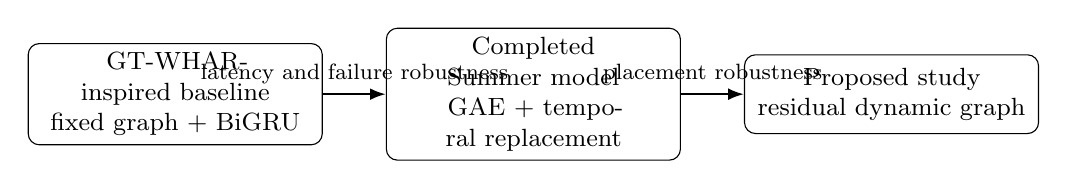
\begin{tikzpicture}[
  node distance=0.8cm,
  box/.style={draw,rounded corners,align=center,minimum height=1cm,text width=3.5cm,font=\small},
  arrow/.style={-{Latex[length=2mm]},thick}
]
\node[box] (base) {GT-WHAR-inspired baseline\\fixed graph + BiGRU};
\node[box,right=of base] (summer) {Completed Summer model\\GAE + temporal replacement};
\node[box,right=of summer] (proposed) {Proposed study\\residual dynamic graph};
\draw[arrow] (base)--node[above,font=\footnotesize]{latency and failure robustness}(summer);
\draw[arrow] (summer)--node[above,font=\footnotesize]{placement robustness}(proposed);
\end{tikzpicture}
\caption{Research progression from the summer baseline to the proposed study.}
\label{fig:progression}
\end{figure}

\section{Datasets Used in the Summer Study}
The summer report uses DSADS, OPPORTUNITY and REALDISP~\cite{summerreport}. DSADS provides five body-worn IMUs and 19 activities. The selected OPPORTUNITY setting tests short and imbalanced activities. REALDISP contains nine IMUs and 33 activities. However, the reported REALDISP experiment focuses on ideal placement rather than the self-placement and induced-displacement scenarios needed for the present research question.

\section{Reported Observations}
The report presents the following completed observations:
\begin{itemize}
\item a large reduction in batch-level GPU inference time after the temporal replacement;
\item similar clean recognition performance between the graph--BiGRU baseline and the proposed summer model; and
\item improved recognition under simulated one- and two-sensor failures when reconstruction and sensor-drop training are used.
\end{itemize}

Table~\ref{tab:summer-evidence} separates completed evidence from conclusions that remain unsupported.

\begin{table}[hbt!]
\centering
\small
\renewcommand{\arraystretch}{1.3}
\caption{Status of the evidence inherited from the Summer Colloquium.}
\label{tab:summer-evidence}
\begin{tabularx}{\textwidth}{@{}P{0.27\textwidth}P{0.31\textwidth}Y@{}}
\toprule
\textbf{Aspect} & \textbf{Completed evidence} & \textbf{Boundary for the proposed study} \\
\midrule
Temporal efficiency & Batch-level GPU timing was reported for baseline and replacement. & Reconcile configurations and measure batch-one end-to-end latency. \\
Missing sensors & Artificially removed sensor streams were tested. & A missing sensor is not a displaced but active sensor. \\
Graph reconstruction & A decoder and joint loss were trained. & Its classification benefit requires a controlled ablation. \\
REALDISP & Ideal-placement activity recognition was reported. & Self/induced placement robustness remains untested. \\
Graph topology & Fixed anatomical graph used throughout. & Input-adaptive routing is proposed for the present work. \\
\bottomrule
\end{tabularx}
\end{table}

\section{Limitations Inherited by the Proposed Study}
The completed project leaves four issues that must be handled before the dynamic-graph claim is tested:
\begin{enumerate}
\item preprocessing and normalization must be fitted using training subjects only;
\item historical metrics must be linked to exact configurations, seeds, checkpoints and batch sizes;
\item the temporal block must be described according to its actual recurrence; and
\item fixed topology, ideal placement and simulated sensor failure do not demonstrate placement robustness.
\end{enumerate}

\section{Transition to the Proposed Study}
The proposed study retains the summer model as the project baseline but changes only the spatial routing first. The temporal backbone and classifier are held fixed during the main graph comparison. This isolates whether adaptive edges, rather than a simultaneous temporal or loss change, explain any robustness difference.

\cleardoublepage
\chapter[Problem Statement and Formulation]{Problem Statement and\\Formulation}

This chapter defines placement variation, states the research question mathematically and specifies the requirements, assumptions and hypotheses of the proposed study.

\section{Types of Sensor Variability}
Figure~\ref{fig:shift-types} distinguishes the four conditions considered in the project.

\begin{figure}[hbt!]
\centering
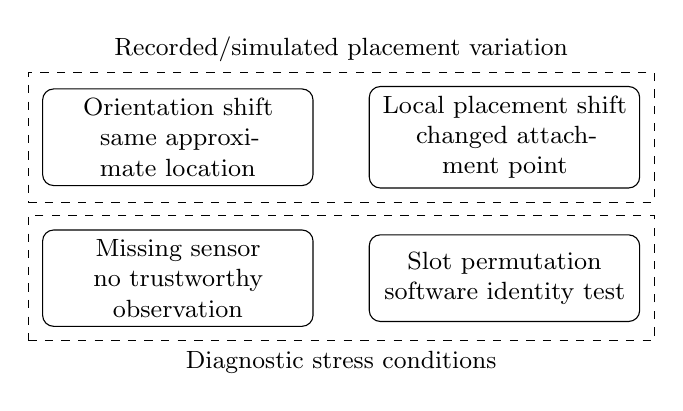
\begin{tikzpicture}[
  box/.style={draw,rounded corners,align=center,minimum height=1.1cm,text width=3.2cm,font=\small},
  node distance=0.55cm and 0.7cm
]
\node[box] (rot) {Orientation shift\\same approximate location};
\node[box,right=of rot] (trans) {Local placement shift\\changed attachment point};
\node[box,below=of rot] (miss) {Missing sensor\\no trustworthy observation};
\node[box,right=of miss] (perm) {Slot permutation\\software identity test};
\node[draw,dashed,fit=(rot)(trans),inner sep=5pt,label=above:{\small Recorded/simulated placement variation}] {};
\node[draw,dashed,fit=(miss)(perm),inner sep=5pt,label=below:{\small Diagnostic stress conditions}] {};
\end{tikzpicture}
\caption{Placement and availability conditions are evaluated separately.}
\label{fig:shift-types}
\end{figure}

Orientation changes rotate the coordinate frame of vector measurements. Local placement shifts change the motion observed at the device. Missing sensors remove information. Slot permutations are useful for diagnosing order dependence but do not reproduce the physics of displacement.

\section{Formal Task}
For one window, let
\[
X=[X_1,\ldots,X_N]\in\mathbb{R}^{T\times N\times F},
\qquad y\in\{1,\ldots,C\},
\]
where $X_i$ is the signal of sensor $i$ and $C$ is the activity count. Availability vector $m\in\{0,1\}^{N}$ indicates whether each sensor is observed. A model $f_\theta$ predicts
\[
\hat y=f_\theta(X,m).
\]
$T$ is the number of samples in the window, $N$ is the number of sensors, $F$ is the number of features per sensor, $y$ is the true activity label, $\hat y$ is the predicted label, $f_\theta$ is the classifier and $\theta$ denotes all trainable model parameters.

Let $P_0$ denote ideal-placement data and $P_s$ a shifted placement condition. The robustness objective is not only high $F_1(P_s)$, but limited degradation
\[
\Delta F_1=F_1(P_0)-F_1(P_s),
\]
where $F_1(P_0)$ is macro-F1 on ideal-placement distribution $P_0$, $F_1(P_s)$ is macro-F1 on shifted distribution $P_s$, and $\Delta F_1$ is the resulting placement degradation. The aim is to limit $\Delta F_1$ while maintaining acceptable clean performance and inference cost.

\section{Why a Fixed Graph Can Fail}
With a fixed adjacency $A_{\mathrm{phys}}$, a graph layer applies the same neighbourhood structure to every window:
\[
H^{(\ell+1)}=\sigma\!\left(A_{\mathrm{phys}}H^{(\ell)}W^{(\ell)}\right).
\]
Here, $A_{\mathrm{phys}}$ is the fixed anatomical adjacency, $H^{(\ell)}$ and $H^{(\ell+1)}$ are the input and output node features of layer $\ell$, $W^{(\ell)}$ is a learned transformation and $\sigma(\cdot)$ is the activation function. If placement changes the meaning or reliability of a node's features, the same messages continue to be propagated. The graph may amplify misleading evidence because its edge strengths cannot respond to the current sample.

A purely dynamic graph $A(X)$ can respond to observations but may overfit activity-specific correlations or become unstable when displacement data are scarce. The proposed solution therefore combines the fixed prior with learned corrections.

\section{Problem Statement}
The problem addressed is:
\begin{quote}
Given multi-IMU activity windows from unseen subjects, develop and evaluate a placement-aware graph model that adapts inter-sensor information flow under recorded orientation and local placement variations, while preserving useful ideal-placement performance and practical inference cost.
\end{quote}

The research question is:
\begin{quote}
Does residual input-dependent and availability-aware routing reduce placement-induced macro-F1 degradation beyond a corrected fixed graph, simple augmentation and DynamicWHAR under a matched subject-independent protocol?
\end{quote}

\section{System Requirements}
The proposed study imposes five requirements:
\begin{enumerate}
\item \textbf{Attribution:} only spatial routing changes during the first comparison.
\item \textbf{Validity:} test subjects and scenarios do not influence normalization or tuning.
\item \textbf{Stability:} graph rows remain finite under masking and edge gradients are preserved.
\item \textbf{Efficiency:} graph generation is included in latency and memory measurements.
\item \textbf{Bounded claims:} dynamic routing does not imply online weight updates or guaranteed anatomical relabelling.
\end{enumerate}

\section{Research Hypotheses}
The proposal tests three hypotheses:
\begin{itemize}
\item \textbf{H1:} Input-dependent routing reduces real-placement degradation relative to a matched fixed graph.
\item \textbf{H2:} A physical prior plus adaptive corrections is more stable than a purely learned dynamic graph.
\item \textbf{H3:} Availability-aware routing improves missing-sensor robustness without a large ideal-placement penalty.
\end{itemize}

\section{Modelling Assumptions}
The primary task is observed-window-end classification. Sensors have known identities in the standard input layout. Training uses labelled source-subject activities. Real displaced test recordings are not used for hyperparameter selection. Arbitrary body-location discovery is not assumed. Negative results are reported if dynamic routing does not improve the matched baseline.

\cleardoublepage
\chapter[Literature Review and Research Gap]{Literature Review and\\Research Gap}

This chapter reviews only the papers central to the proposed work: DeepConvLSTM as the sequence baseline, GT-WHAR and GIN as the graph foundation, DynamicWHAR as the direct wearable dynamic-interaction baseline, 2s-AGCN as the residual adaptive-graph foundation, Mamba and DecomposeWHAR as temporal and cross-sensor prior art, and the REALDISP displacement study as the evaluation foundation.

\section{Deep Sequence Modelling}
DeepConvLSTM combines convolutional layers with LSTM recurrence for multimodal wearable activity recognition~\cite{deepconvlstm}.
\begin{itemize}
\item \textbf{Method:} convolutions extract local temporal patterns and recurrent layers integrate information across the complete input window.
\item \textbf{Relevance:} it provides a strong non-graph sequence baseline and tests whether explicit graph structure is useful.
\item \textbf{Limitation:} sensor relations remain implicit in channel order and learned filters, so robustness to changed placement is not built into the architecture.
\end{itemize}

\section{GIN and GT-WHAR}
GIN was proposed as an expressive graph neural network based on injective neighbourhood aggregation~\cite{gin}. A common form is
\[
h_v^{(k)}=\operatorname{MLP}^{(k)}
\left((1+\epsilon^{(k)})h_v^{(k-1)}+
\sum_{u\in\mathcal N(v)}h_u^{(k-1)}\right).
\]
GT-WHAR applies graph and temporal modelling to multiple wearable sensors~\cite{gtwhar}. It provides the literature foundation for the summer baseline and for retaining explicit sensor nodes. However, the project implementation uses a fixed anatomical graph. The current proposal asks whether weighted adaptive edges improve robustness under placement shift.

In the GIN expression, $h_v^{(k)}$ is the representation of node $v$ after layer $k$, $h_u^{(k-1)}$ is the previous representation of neighbouring node $u$, $\mathcal N(v)$ is the neighbourhood of $v$, $\epsilon^{(k)}$ controls the self-node contribution, and $\operatorname{MLP}^{(k)}$ is the trainable multilayer perceptron at layer $k$. The paper's role in this work is:
\begin{itemize}
\item \textbf{Method:} expressive graph aggregation followed by temporal modelling of wearable signals.
\item \textbf{Relevance:} foundation of the completed fixed-graph system and the internal baseline.
\item \textbf{Limitation:} fixed anatomical routing cannot alter edge strengths for each observed placement condition.
\end{itemize}

\section{DynamicWHAR}
DynamicWHAR learns dynamic inter-sensor correlations after extracting features for individual wearable sensors~\cite{dynamicwhar}.
\begin{itemize}
\item \textbf{Method:} estimate pairwise interactions from per-sensor latent representations and aggregate complementary information according to the current sample.
\item \textbf{Relevance:} closest direct external baseline for dynamic wearable-sensor interaction.
\item \textbf{Limitation:} it does not by itself establish the benefit of a residual anatomical prior under the proposed matched REALDISP protocol.
\end{itemize}
Consequently, the gap is not that dynamic graphs are absent from WHAR. The question is whether physical, globally learned and sample-dependent branches provide additional placement robustness in the inherited system.

\section{2s-AGCN}
The two-stream adaptive graph convolutional network was proposed for skeleton-based action recognition~\cite{agcn}.
\begin{itemize}
\item \textbf{Method:} combine a fixed physical graph, a globally learned graph and a sample-specific graph.
\item \textbf{Relevance:} motivates retaining anatomical structure while learning global and input-dependent corrections.
\item \textbf{Limitation:} its nodes are visual skeleton joints; wearable IMUs require temporal sensor embeddings, availability masks and direct placement evaluation.
\end{itemize}
The proposed graph therefore adapts the residual principle rather than claiming a direct reproduction of 2s-AGCN.

\section{Mamba and DecomposeWHAR}
\begin{itemize}
\item \textbf{Mamba:} uses input-dependent selective state-space parameters for efficient sequence modelling~\cite{mamba}. It provides a temporal reference but does not define a body-sensor graph or placement-invariance mechanism.
\item \textbf{DecomposeWHAR:} combines modality-aware decomposition, SSM temporal aggregation and dynamic cross-sensor self-attention~\cite{decompose}. It proves that SSM processing and dynamic sensor fusion already coexist.
\item \textbf{Implication:} novelty must be supported by the placement-specific residual routing design and matched evaluation, not merely by combining Mamba with attention or a graph.
\end{itemize}

\section{REALDISP and Sensor Displacement}
REALDISP was developed to evaluate activity recognition under realistic sensor displacement~\cite{realdisp,banos}.
\begin{itemize}
\item \textbf{Methodological role:} distinguish ideal placement, self-placement and induced displacement instead of replacing physical displacement with channel permutations.
\item \textbf{Why it matters:} placement can change vector orientation, local motion and inter-sensor relationships even when every device remains active.
\item \textbf{Protocol constraint:} induced displacement is documented for subjects 2, 5 and 15, so unavailable subject--scenario pairs cannot be treated as full 17-subject folds~\cite{banos}.
\end{itemize}

\section{Literature Synthesis}
Table~\ref{tab:literature-summary} summarises the core works and the precise scope taken from each.

\begin{table}[hbt!]
\centering
\small
\renewcommand{\arraystretch}{1.3}
\caption{Core literature and the scope derived for this project.}
\label{tab:literature-summary}
\begin{tabularx}{\textwidth}{@{}P{0.25\textwidth}P{0.25\textwidth}Y@{}}
\toprule
\textbf{Work} & \textbf{Main contribution} & \textbf{Role and boundary} \\
\midrule
DeepConvLSTM~\cite{deepconvlstm} & CNN--LSTM wearable sequence baseline. & Non-graph control; sensor topology remains implicit. \\
GIN / GT-WHAR~\cite{gin,gtwhar} & Expressive graph aggregation and graph--temporal wearable modelling. & Fixed-graph project foundation and continuity. \\
DynamicWHAR~\cite{dynamicwhar} & Dynamic pairwise wearable sensor interactions. & Mandatory external dynamic baseline; prevents an overbroad novelty claim. \\
2s-AGCN~\cite{agcn} & Physical, learned and sample-adaptive graph components. & Residual graph principle; skeleton inputs differ from wearable IMUs. \\
Mamba~\cite{mamba} & Selective state-space temporal modelling. & Temporal reference; does not solve displacement alone. \\
DecomposeWHAR~\cite{decompose} & SSM aggregation with dynamic cross-sensor attention. & Essential graph/SSM prior art and comparator where feasible. \\
REALDISP study~\cite{banos,realdisp} & Recorded ideal, self and induced placement conditions. & Primary displacement evidence and protocol constraint. \\
\bottomrule
\end{tabularx}
\end{table}

\section{Research Gaps and Proposed Novelty}
The literature yields four gaps:
\begin{enumerate}
\item \textbf{Project evidence gap:} the completed summer work does not evaluate real placement robustness.
\item \textbf{Matched-comparison gap:} dynamic interaction exists, but its benefit relative to the corrected inherited model and simple augmentation is unknown under one protocol.
\item \textbf{Mechanism gap:} the contributions of physical, global and sample-dependent graph branches have not been isolated for this system.
\item \textbf{Evaluation gap:} the project lacks a traceable comparison across recorded placement, missing sensors and efficiency using the same subjects, inputs and tuning budget.
\end{enumerate}

The research-gap statement is:
\begin{quote}
Although dynamic inter-sensor learning, adaptive graph construction and state-space temporal modelling already exist, their benefit for the inherited fixed-graph GAE--temporal system under a matched real-displacement protocol is not established. This work will test whether residual placement-aware routing provides robustness beyond fixed graphs, augmentation and DynamicWHAR.
\end{quote}
\vspace{-5pt}

The intended novelty is evidence-driven: a residual placement-aware routing mechanism integrated with the inherited system and evaluated through controlled graph-branch, masking and reconstruction ablations. The adjacency formula alone is not treated as sufficient novelty.

\cleardoublepage
\chapter[Methodological Foundations and Proposed Approach]{Methodological Foundations\\and Proposed Approach}

This chapter explains the methodology of the most important papers and then derives the proposed model. The purpose is to show exactly which ideas are retained, which are adapted and which claims remain to be tested.

\section{Methodology of GT-WHAR}
GT-WHAR represents multiple wearable sensors as graph nodes, applies graph-based spatial modelling and then captures temporal structure~\cite{gtwhar}. Its methodology is transferred as follows:
\begin{itemize}
\item \textbf{Input representation:} preserve one node representation per physical sensor.
\item \textbf{Spatial stage:} exchange information through graph message passing.
\item \textbf{Temporal stage:} model the sequence after spatial aggregation.
\item \textbf{Project use:} retain spatial--temporal separation, but replace fixed routing with a controlled adaptive alternative.
\end{itemize}

The corrected fixed-graph version of the inherited model is the main internal baseline. This report does not claim an exact reproduction unless the official architecture, inputs and protocol are matched.

\section{Methodology of DynamicWHAR}
DynamicWHAR proceeds in three main stages~\cite{dynamicwhar}:
\begin{enumerate}
\item encode each wearable sensor separately to obtain a stable sensor-level representation;
\item estimate sample-conditioned interaction intensity between sensor pairs; and
\item aggregate interaction features for activity classification.
\end{enumerate}
For this project, affinities are therefore computed from per-sensor latent features rather than raw heterogeneous channels. DynamicWHAR is also retained as the required external dynamic-interaction control.

\section{Methodology of 2s-AGCN}
In 2s-AGCN, graph convolution uses a sum of physical, trainable and sample-dependent adjacency components~\cite{agcn}. In simplified notation,
\[
Y=\sum_k W_kX(A_k+B_k+C_k),
\]
where $k$ indexes graph partitions, $X$ is the input feature tensor, $Y$ is the graph-convolution output, $W_k$ is the trainable transformation for partition $k$, $A_k$ is the predefined physical adjacency, $B_k$ is a dataset-level learned adjacency and $C_k$ is the current-sample adjacency. The physical graph anchors training, while adaptive components capture relations not represented by the predefined skeleton.

The proposed model transfers this residual principle to IMUs. Unlike skeleton joints, each IMU supplies a short multivariate time series. A per-sensor encoder is therefore required before graph construction, and missing sensors require an explicit mask.

\section[Methodology of Mamba and DecomposeWHAR]{Methodology of Mamba and\\DecomposeWHAR}
A continuous state-space model can be written as
\[
\dot h(t)=Ah(t)+Bx(t),\qquad y(t)=Ch(t).
\]
Here, $t$ is continuous time, $x(t)$ is the input, $h(t)$ is the latent state, $\dot h(t)$ is its time derivative, $y(t)$ is the output, and $A$, $B$ and $C$ are state-transition, input and output matrices. After discretisation, the state is updated along a sequence. Mamba makes selected state-space parameters input-dependent and implements the recurrence efficiently~\cite{mamba}. The defining contribution is selective recurrence, not the use of a convolution or gate alone.

DecomposeWHAR separates intra-sensor modality processing from inter-sensor fusion, uses Mamba-like SSM processing for long-range temporal dependencies and applies dynamic cross-sensor self-attention~\cite{decompose}. The present proposal adopts the methodological separation between per-sensor encoding, temporal modelling and cross-sensor interaction, but uses an explicit residual graph to retain anatomical structure.

\section{Proposed System Architecture}
Figure~\ref{fig:proposed-architecture} shows the proposed pipeline.

\begin{figure}[hbt!]
\centering
\resizebox{\textwidth}{!}{%
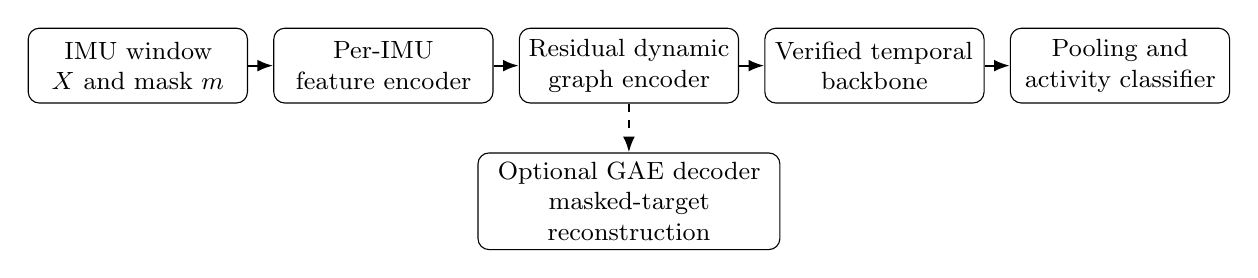
\begin{tikzpicture}[
  node distance=0.32cm,
  box/.style={draw,rounded corners,align=center,minimum height=0.95cm,text width=2.55cm,font=\small},
  arrow/.style={-{Latex[length=2mm]},thick}
]
\node[box] (input) {IMU window\\$X$ and mask $m$};
\node[box,right=of input] (embed) {Per-IMU\\feature encoder};
\node[box,right=of embed] (graph) {Residual dynamic\\graph encoder};
\node[box,right=of graph] (temp) {Verified temporal\\backbone};
\node[box,right=of temp] (head) {Pooling and\\activity classifier};
\node[box,below=0.62cm of graph,text width=3.6cm] (decoder) {Optional GAE decoder\\masked-target reconstruction};
\draw[arrow] (input)--(embed);
\draw[arrow] (embed)--(graph);
\draw[arrow] (graph)--(temp);
\draw[arrow] (temp)--(head);
\draw[arrow,dashed] (graph)--(decoder);
\end{tikzpicture}
}
\caption{Proposed placement-aware graph--temporal pipeline. The decoder is auxiliary.}
\label{fig:proposed-architecture}
\end{figure}

\subsection{Per-Sensor Feature Encoding}
For each IMU $i$, a lightweight temporal encoder produces
\[
H_i=\phi(X_i)\in\mathbb{R}^{T'\times d}.
\]
Here, $i\in\{1,\ldots,N\}$ identifies the IMU, $X_i\in\mathbb{R}^{T\times F}$ is its input window, $\phi(\cdot)$ is the temporal feature encoder, $H_i$ is the resulting embedding sequence, $T'$ is its temporal length and $d$ is the embedding dimension. The same encoder structure is applied to each sensor, with location identity retained separately. Feature normalization controls scale before affinity computation. The encoder is not assumed to remove all sensor noise.

\subsection{Residual Dynamic Adjacency}
At temporal index $t$, let $H_t\in\mathbb{R}^{N\times d}$ contain the sensor embeddings. Sample-dependent affinity is
\[
Q_t=H_tW_Q,\qquad K_t=H_tW_K,
\]
\[
C_t=\operatorname{softmax}_{\mathrm{row}}
\left(\frac{Q_tK_t^{\top}}{\tau\sqrt d}\right),
\]
where $t$ is the temporal index, $H_t\in\mathbb{R}^{N\times d}$ contains all sensor embeddings at $t$, $W_Q$ and $W_K$ are trainable projections, $Q_t$ and $K_t$ are query and key matrices, $d$ is the embedding dimension, $\tau>0$ is a temperature and row-wise softmax converts affinities into normalized outgoing weights. The residual graph is
\[
\widetilde A_t=
\alpha_tA_{\mathrm{phys}}
+\beta_tA_{\mathrm{global}}
+\gamma_tC_t
+\delta I_N,
\]
\[
A_t=\operatorname{RowNorm}
\left(M_t\odot\operatorname{ReLU}(\widetilde A_t)+\varepsilon I_N\right).
\]
$\widetilde A_t$ is the unnormalized mixture; $A_{\mathrm{phys}}$ is the anatomical prior; $A_{\mathrm{global}}$ is a nonnegative trainable matrix; $C_t$ is sample-dependent; $I_N$ is the $N\times N$ identity matrix; and $\alpha_t$, $\beta_t$, $\gamma_t$ and $\delta$ are nonnegative mixture weights. $\operatorname{ReLU}$ removes negative edge values, $\odot$ denotes element-wise multiplication, $M_t$ is the availability mask, $\varepsilon>0$ protects empty rows, and $\operatorname{RowNorm}$ divides every row by its sum to obtain $A_t$. The gates are initialized to favour the physical branch without permanently forcing it.

For sender availability $m_j$,
\[
(M_t)_{ij}=m_j.
\]
Here, $i$ is the receiving sensor, $j$ is the sending sensor and $m_j\in\{0,1\}$ indicates whether sender $j$ is available. Thus every edge originating from an unavailable sender is suppressed. A learned reliability score is postponed until the basic graph comparison identifies a need for it.

\begin{figure}[hbt!]
\centering
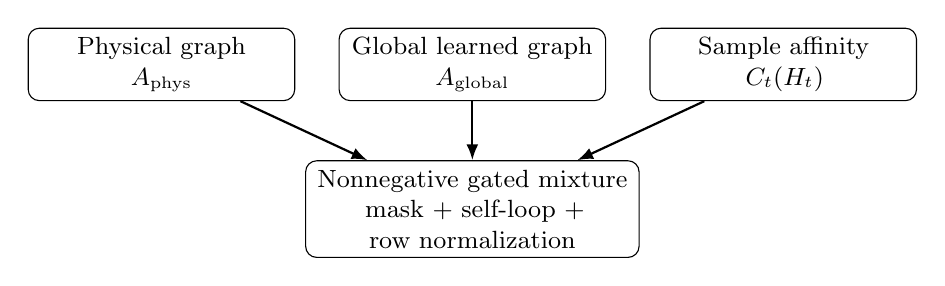
\begin{tikzpicture}[
  box/.style={draw,rounded corners,align=center,minimum height=0.9cm,text width=3.15cm,font=\small},
  arrow/.style={-{Latex[length=2mm]},thick},
  node distance=0.55cm
]
\node[box] (phys) {Physical graph\\$A_{\mathrm{phys}}$};
\node[box,right=of phys] (global) {Global learned graph\\$A_{\mathrm{global}}$};
\node[box,right=of global] (dynamic) {Sample affinity\\$C_t(H_t)$};
\node[box,below=0.75cm of global,text width=4cm] (mix) {Nonnegative gated mixture\\mask + self-loop + row normalization};
\draw[arrow] (phys)--(mix);
\draw[arrow] (global)--(mix);
\draw[arrow] (dynamic)--(mix);
\end{tikzpicture}
\caption{Three graph branches used by the proposed residual adjacency.}
\label{fig:graph-branches}
\end{figure}

\subsection{Weighted Message Passing}
One graph layer computes
\[
Z_t=\sigma\!\left(A_tH_tW_g+b_g\right)+H_tW_r,
\]
where $Z_t$ is the graph-layer output, $A_t$ is the normalized dynamic adjacency, $H_t$ is the sensor-feature matrix, $W_g$ and $b_g$ are the message transformation and bias, $\sigma(\cdot)$ is a nonlinear activation and $W_r$ is the residual projection. Since the selected datasets contain few sensors, dense batched matrix multiplication is practical and keeps edge gradients. Self-contributions are counted once.

\subsection{Temporal Modelling and Classification}
Graph features are passed to the same verified temporal backbone for all spatial variants. Pooling produces one representation per window, followed by an activity classifier. During the principal experiment, temporal architecture, classifier, augmentation budget and optimizer are held fixed.

\subsection{Optional Reconstruction Branch}
If the GAE is retained, artificially masked clean training windows provide reconstruction targets. The decoder is auxiliary; it is removed in a matched ablation. Real ideal and displaced recordings are not treated as aligned reconstruction pairs unless alignment is demonstrated.

\section{Training Objective}
The proposed objective is
\[
\mathcal L=
\mathcal L_{\mathrm{cls}}
+\lambda_{\mathrm{rec}}\mathcal L_{\mathrm{rec}}
+\lambda_{\mathrm{edge}}\mathcal R(A),
\]
Here, $\mathcal L$ is the total training loss, $\mathcal L_{\mathrm{cls}}$ is activity-classification loss, $\mathcal L_{\mathrm{rec}}$ is reconstruction loss computed only on intentionally masked targets, $\mathcal R(A)$ is an optional regularizer over the learned adjacency sequence $A$, and $\lambda_{\mathrm{rec}}$ and $\lambda_{\mathrm{edge}}$ are their nonnegative weights. The no-decoder control uses $\lambda_{\mathrm{rec}}=0$.

\section{Implementation Stability}
Potential graph failures include uniform attention, one-hot attention, over-smoothing and invalid normalization for fully masked rows. The implementation will use scaled logits, normalized sensor embeddings, finite-value checks, residual paths and logged branch weights. Top-$k$ sparsification is evaluated only as an ablation.

\section{Planned Ablations}
\begin{table}[hbt!]
\centering
\small
\renewcommand{\arraystretch}{1.3}
\caption{Design choices and matched alternatives.}
\label{tab:design-ablation}
\begin{tabularx}{\textwidth}{@{}P{0.29\textwidth}Y@{}}
\toprule
\textbf{Variant} & \textbf{Question answered} \\
\midrule
No graph / fixed physical graph & Is explicit graph structure useful and what is the corrected baseline? \\
Normalized static graph & Is a gain caused only by changed aggregation scale? \\
Global learned branch only & Is a sample-independent learned topology sufficient? \\
Dynamic affinity only & Does unrestricted sample-dependent routing become unstable? \\
Physical + global + dynamic & Does the residual mixture give the best robustness--clean trade-off? \\
With/without availability mask & Does explicit missingness handling help? \\
With/without GAE loss & Does reconstruction improve recognition? \\
Rotation augmentation only & Can a simple data-level method explain the gain? \\
\bottomrule
\end{tabularx}
\end{table}

\cleardoublepage
\chapter[Datasets and Evaluation Methodology]{Datasets and Evaluation\\Methodology}

This chapter defines the datasets, preprocessing, baselines, metrics and experimental protocol that will be fixed before final testing. The dynamic graph remains proposed work; this chapter specifies how it will be evaluated rather than presenting new results.

\section{Datasets}

\subsection{REALDISP}
REALDISP is the primary dataset because it records placement variability~\cite{realdisp,banos}. The UCI record lists 1,419 instances distributed across 47 files, 17 subjects, 33 activities and nine IMUs sampled at 50 Hz. The devices are positioned on the left/right calves, thighs, lower arms and upper arms, with one sensor on the back. Each raw row contains two timestamps, 13 channels from each IMU and an activity label: tri-axial acceleration, angular velocity and magnetic field plus a four-component orientation quaternion. The full row therefore has 120 attributes. The proposed starting input uses the nine acceleration/gyroscope/magnetometer channels per sensor; initial windows use $T=50$ and stride 25, subject to verification against the raw files and baseline protocol.

The dataset documents ideal placement, self-placement and induced displacement. Scenario availability must be audited: induced displacement is reported for subjects 2, 5 and 15~\cite{banos}. The evaluation will use only valid subject--scenario pairs and will state exclusions explicitly.

\subsection{DSADS}
DSADS contains 9,120 labelled five-second segments from eight subjects performing 19 activities~\cite{dsads}. Five Xsens units are attached to the torso, right arm, left arm, right leg and left leg. Every activity is recorded in 60 segments per subject at 25 Hz; each segment contains 125 rows and 45 signal columns, corresponding to five sensors with nine acceleration, gyroscope and magnetic-field axes each. It provides a secondary cross-subject benchmark for controlled rotation and sensor-drop experiments but does not replace REALDISP's recorded displacement evidence.

\subsection{OPPORTUNITY}
OPPORTUNITY is retained only as a supplementary inherited dataset~\cite{opportunity}. It records four users completing six runs each, giving 24 runs: five activities-of-daily-living runs and one drill run per user. The complete body-worn setup includes seven IMUs, twelve three-dimensional acceleration sensors and four three-dimensional localization tags, in addition to object and ambient sensors. The repository lists 88 files. Its short gestures and strong Null-class imbalance may test generalisation after the REALDISP study is stable. The exact project sensor subset, activity labels and Null-class policy will be declared; a selected five-IMU input is not described as the complete dataset.

\begin{table}[hbt!]
\centering
\small
\renewcommand{\arraystretch}{1.3}
\caption{Datasets and their roles in the proposed evaluation.}
\label{tab:datasets}
\begin{tabularx}{\textwidth}{@{}P{0.20\textwidth}P{0.27\textwidth}Y@{}}
\toprule
\textbf{Dataset} & \textbf{Starting configuration} & \textbf{Role} \\
\midrule
REALDISP & 1,419 UCI instances; 47 files; 17 subjects; 9 IMUs; 33 activities; 50 Hz; 120 raw attributes. & Primary recorded placement evaluation; audit scenario availability. \\
DSADS & 9,120 segments; 8 subjects; 5 IMUs; 19 activities; 25 Hz; $125\times45$ per segment. & Secondary subject-generalisation and synthetic stress evaluation. \\
OPPORTUNITY & 4 users; 24 runs; 7 body IMUs plus other body, object and ambient sensors; 88 files. & Optional supplementary study using an explicitly declared subset and label policy. \\
\bottomrule
\end{tabularx}
\end{table}

\section{Data Audit and Preprocessing}
Every raw recording is entered in a manifest containing subject, session, scenario, timestamps, labels and sensor/channel order. Units, sampling rates, missing files, NaNs and class counts are verified. Subjects are divided before windowing and normalization. Training means and variances are fitted only from training subjects.

Synthetic rotations are applied in raw units. All vector modalities from one IMU receive a consistent rotation within a window. Dropout, noise and rotation severities are recorded separately. Slot permutation is used only as a diagnostic order-sensitivity test.

\section{Subject-Independent Split}
The intended outer protocol is leave-one-subject-out where scenario availability permits. For each outer test subject, a separate source subject is used for validation. Training uses source-subject ideal recordings and declared synthetic corruptions. Hyperparameters and checkpoint selection use validation data only.

Because induced displacement has limited subject coverage, it is reported as a targeted paired evaluation rather than averaged over unavailable folds. Self-placement supports a broader analysis after its file availability is verified. All methods are compared on the same subject--scenario pairs.

\section{Baselines}
The minimum baseline set is:
\begin{enumerate}
\item DeepConvLSTM or a compact CNN/TCN sequence model;
\item no-graph version of the inherited temporal system;
\item corrected fixed anatomical graph, with and without GAE reconstruction;
\item fixed graph with rotation/dropout augmentation;
\item DynamicWHAR under the common protocol; and
\item the proposed residual dynamic graph.
\end{enumerate}
DecomposeWHAR is included if its input and split can be matched. Published scores from incompatible protocols are discussed but not inserted into a direct result table.

\section{Evaluation Conditions}
The following conditions are reported separately:
\begin{itemize}
\item ideal placement;
\item self-placement and available induced displacement;
\item synthetic per-IMU rotation;
\item one- and multi-sensor dropout; and
\item combined placement and dropout stress after individual effects are understood.
\end{itemize}

\section{Metrics}
The primary metric is subject-level macro-F1. Accuracy and weighted F1 are secondary. Robustness is summarised by clean-to-shift degradation $\Delta F_1$. Reports include per-class F1, worst-subject performance, confusion matrices and sensor/scenario-specific failures.

Efficiency includes parameter count, peak memory, batch-one median and p95 latency, and the input-window duration/stride. The device, software, precision and synchronization method are reported. Batch-level GPU throughput is not equated with edge-device latency.

\section{Experimental Protocol}
The architecture and hyperparameters are selected using training and validation subjects. After the design is frozen, all available outer test folds are run. Selected methods use multiple seeds where compute permits. Seed predictions are averaged within subjects before paired comparison. Confidence intervals are formed by resampling subjects or valid paired subject--scenario units.

Negative results and harmed classes are retained. A routing gain is considered meaningful only if it exceeds seed variation, improves shifted performance beyond augmentation and does not create an unacceptable ideal-placement loss.

\section{Expected Evidence after Prototype Development}
The implementation review should contain an executable baseline, a reproduced or documented DynamicWHAR control, a functioning weighted graph, branch ablations, preliminary validation results and measured inference overhead. It should not present test-set tuning or claim state of the art from unmatched literature scores.

\cleardoublepage
\chapter{Conclusion and Future Work}

This chapter summarises the completed and proposed work, states the present limitations and defines the immediate path from proposal to implementation and final evaluation.

\section{Conclusion}
The completed Summer Colloquium moved from a GT-WHAR-inspired graph--BiGRU baseline to GAE--Mamba--WHAR, addressing batch-level temporal cost and simulated missing sensors. It did not establish robustness to a present but displaced sensor. The fixed-topology limitation motivates the proposed study.

The proposed work combines a physical graph, a globally learned graph and a sample-dependent affinity graph. Availability masking prevents messages from missing senders. The temporal backbone remains fixed during the main graph comparison, and the GAE is retained only if ablation supports it. REALDISP provides the primary real-placement evidence, with DSADS as secondary support.

The contribution will be judged through matched evidence rather than architectural labels: whether residual routing improves placement robustness, which graph branches cause the effect, what clean-performance cost is incurred and what inference overhead is added.

\section{Current Limitations}
At this proposal stage, no dynamic-graph performance result exists. Additional limitations are:
\begin{itemize}
\item induced REALDISP displacement covers a limited set of subjects;
\item learned affinity may capture activity correlations rather than true placement changes;
\item dynamic routing cannot automatically infer an unknown anatomical location;
\item synthetic rotation and dropout are controls, not substitutes for recorded displacement;
\item the GAE may regularise features without reconstructing a physically correct trajectory; and
\item deployment feasibility requires batch-one profiling on a named device.
\end{itemize}

\section{Immediate Implementation Work}
The immediate tasks are:
\begin{enumerate}
\item recover and audit the summer code, splits, preprocessing, checkpoints and logs;
\item reproduce a corrected fixed-graph pilot and no-graph control;
\item reproduce DynamicWHAR or document remaining reproduction gaps;
\item implement weighted graph branches, masking and gradient/finite-value tests;
\item compare fixed, augmentation and adaptive variants on validation subjects; and
\item complete graph, mask and reconstruction ablations before freezing the final experiments.
\end{enumerate}

\section{Future Work}
Future work will complete the locked REALDISP evaluation, add DSADS generalisation, run final seeds and uncertainty analysis, and choose one extension based on observed failure evidence. If present but unreliable sensors remain the main error, reliability-aware routing will be studied. If orientation remains dominant, rotation-equivariant per-IMU encoding may be considered. Unrelated additions will be deferred until the core placement study is complete.

\begin{table}[hbt!]
\centering
\small
\renewcommand{\arraystretch}{1.3}
\caption{Stage-wise deliverables.}
\label{tab:deliverables}
\begin{tabularx}{\textwidth}{@{}P{0.20\textwidth}P{0.42\textwidth}Y@{}}
\toprule
\textbf{Stage} & \textbf{Main work} & \textbf{Deliverables} \\
\midrule
Proposal & Problem, core literature, gap, proposed method and evaluation plan. & Report and presentation; no new result claim. \\
Prototype development & Audited baseline, DynamicWHAR control and dynamic-graph prototype. & Executable code, preliminary validation and ablations. \\
Final evaluation & Locked testing and one justified extension. & Final experiments, efficiency study, reproducible artifacts, thesis and defense. \\
\bottomrule
\end{tabularx}
\end{table}

\section{Closing Statement}
This report defines a focused continuation of the completed Summer Colloquium. It does not restart the project and does not claim that dynamic graphs or SSMs are new. It proposes a controlled placement-aware extension and a protocol capable of determining whether that extension is genuinely useful.

\cleardoublepage
\begin{multicols}{2}
\small
\begin{thebibliography}{99}
\raggedright
\setlength{\itemsep}{3pt}
\setlength{\parskip}{0pt}

\bibitem{deepconvlstm}
F. J. Ord\'o\~nez and D. Roggen,
``Deep Convolutional and LSTM Recurrent Neural Networks for Multimodal Wearable Activity Recognition,''
\emph{Sensors}, vol. 16, no. 1, art. 115, 2016.
\href{https://doi.org/10.3390/s16010115}{doi:10.3390/s16010115}.

\bibitem{gin}
K. Xu, W. Hu, J. Leskovec, and S. Jegelka,
``How Powerful are Graph Neural Networks?''
in \emph{Proc. International Conference on Learning Representations}, 2019.
\href{https://arxiv.org/abs/1810.00826}{arXiv:1810.00826}.

\bibitem{gtwhar}
H. Zou, Z. Chen, J. Zhang, L. Wang, F. Zhang, J. Li, and Y. Pan,
``GT-WHAR: A Generic Graph-Based Temporal Framework for Wearable Human Activity Recognition With Multiple Sensors,''
\emph{IEEE Transactions on Emerging Topics in Computational Intelligence}, vol. 8, no. 6, pp. 3912--3924, 2024.
\href{https://doi.org/10.1109/TETCI.2024.3378331}{doi:10.1109/TETCI.2024.3378331}.

\bibitem{dynamicwhar}
S. Miao, L. Chen, R. Hu, and Y. Luo,
``Towards a Dynamic Inter-Sensor Correlations Learning Framework for Multi-Sensor-Based Wearable Human Activity Recognition,''
\emph{Proceedings of the ACM on Interactive, Mobile, Wearable and Ubiquitous Technologies}, vol. 6, no. 3, art. 130, pp. 1--25, 2022.
\href{https://doi.org/10.1145/3550331}{doi:10.1145/3550331}.

\bibitem{agcn}
L. Shi, Y. Zhang, J. Cheng, and H. Lu,
``Two-Stream Adaptive Graph Convolutional Networks for Skeleton-Based Action Recognition,''
in \emph{Proc. IEEE/CVF Conference on Computer Vision and Pattern Recognition}, 2019, pp. 12026--12035.
\href{https://doi.org/10.1109/CVPR.2019.01230}{doi:10.1109/CVPR.2019.01230}.

\bibitem{mamba}
A. Gu and T. Dao,
``Mamba: Linear-Time Sequence Modeling with Selective State Spaces,''
\emph{Conference on Language Modeling}, 2024; arXiv:2312.00752, 2023.
\href{https://arxiv.org/abs/2312.00752}{arXiv:2312.00752}.

\bibitem{decompose}
H. Xie et al.,
``Decomposing and Fusing Intra- and Inter-Sensor Spatio-Temporal Signal for Multi-Sensor Wearable Human Activity Recognition,''
in \emph{Proc. AAAI Conference on Artificial Intelligence}, vol. 39, no. 13, pp. 14441--14449, 2025.
\href{https://doi.org/10.1609/aaai.v39i13.33582}{doi:10.1609/aaai.v39i13.33582}.

\bibitem{banos}
O. Ba\~nos et al.,
``Dealing with the Effects of Sensor Displacement in Wearable Activity Recognition,''
\emph{Sensors}, vol. 14, no. 6, pp. 9995--10023, 2014.
\href{https://doi.org/10.3390/s140609995}{doi:10.3390/s140609995}.

\bibitem{realdisp}
UCI Machine Learning Repository,
``REAListic Sensor DISPlacement Activity Recognition Dataset (REALDISP),'' 2014.
\href{https://doi.org/10.24432/C5GP6D}{doi:10.24432/C5GP6D}.

\bibitem{dsads}
B. Barshan and K. Altun,
``Daily and Sports Activities,'' UCI Machine Learning Repository, 2013.
\href{https://doi.org/10.24432/C5C59F}{doi:10.24432/C5C59F}.

\bibitem{opportunity}
D. Roggen et al.,
``OPPORTUNITY Activity Recognition,'' UCI Machine Learning Repository, 2012.
\href{https://doi.org/10.24432/C5M027}{doi:10.24432/C5M027}.

\bibitem{summerreport}
P. Kumar,
\emph{GAE-Mamba-WHAR: Generative Kinematic Imputation and Causal State-Space Modeling for Robust Human Activity Recognition},
Summer Colloquium Report, ABV-IIITM Gwalior, August 2026.

\end{thebibliography}
\end{multicols}

\end{document}